\section{数値解析例}
本節では,Na型モンモリロナイトに対する水和エネルギーを用いて行ったCG-MD
シミュレーションの結果を示す.
CG-MD解析では,温度,相対湿度,圧力を一定に保った状態で非平衡状態にある
初期モデルから,モンモリロナイト含水系(以下,粘土含水系と呼ぶ)の
CG-MDモデルで緩和計算を行う.
これを6つの異なる相対湿度において行い,膨潤挙動の観点からみたときの,
シミュレーション結果の妥当性について議論する.
以下,初期モデルと計算手順を述べた後,シミュレーション結果を
粘土分子配置のスナップショットと層間距離の頻度分布を示す。
これらの結果をもとに,相対湿度に応じた膨潤状態の変化について述べる.
\subsection{初期モデルの作成}
緩和計算を行うための初期モデルを図\ref{fig:fig3}-(a)に示す.
これは2021年度の共同研究報告書で述べた方法で作成した粘土含水系モデルの一つで,
粗視化粒子数3,194で構成された,80の粘土分子からなる.
このモデルは以下の手順で作成されている.\\
はじめに,直線状の粘土分子を200$\times$200[nm$^2$]の
矩形領域に互いに重ならないように,位置と向きをランダムに配置する.
この矩形領域を周期構造を構成する単位セルとして,
乾燥密度が約1.6g/cm$^{3}$となるまで1[ns]かけて断熱圧縮する.
その際,粒子系の運動方程式を時間積分するための時間ステップ幅
は0.02[ps],時間ステップ数は5万ステップとしており,
時間積分に関するこの条件は以後の解析でも同じである.
断熱圧縮過程では系の温度を制御していないため,圧縮によって系
に加えれられたエネルギーによって高温になり平衡状態にも無い.
そこで,圧縮後のモデルを300Kまで$250$psをかけて冷却し,
その後750psの間一定温度(300K)で緩和計算を行う.
なお,ここでいう緩和とは,温度や体積などの外的条件を一定にして,
系を平衡状態に向けて推移させることを意味する.
以上の計算では,各粗視化粒子において水分量を表す
パラメータである粒子間相互作用ポテンシャルの特性距離$\sigma$を,
二層膨潤状態に相当する$\sigma=1.5$[nm]に固定し,
系内での水分移動も系外との水分の授受もないものとしている.
最後に,無次元化された化学ポテンシャル$\bar \mu$を$0.5$に保ち,
温度,体積一定のもと,水分分布を含めた緩和計算を1[ns]間行う.
このとき,$\bar \mu$の値は強い排水が起こるように設定されており,
緩和計算後,大きな層外空隙をもつ組織構造が得られる.\\
図\ref{fig:fig3}-(a)は以上の手続きによって得た粘土含水系モデルである.
本年度の研究では,これを初期構造とし,Na型モンモリロナイトの
水和エネルギーモデルを用いて,相対湿度に応じてどのような組織構造
へ移行するか調べる.
初期構造を得るまでの計算では,昨年度の研究で検討を行った
水和エネルギーモデルの一つである振動モデルを用いている.
このモデルは仮想的な粘土の水和挙動を表現したものであるため,
図\ref{fig:fig3}-(a)の状態は,今回新たに作成した水和エネルギーモデル
の下では平衡状態にない.そのため,相対湿度の設定値によらず,
水分や分子配置には必ず何らかの変化が生じる.
\subsection{相対湿度50$\%$に対する結果}
図\ref{fig:fig3}の(b)と(c)は,相対湿度50$\%$,温度300K, 圧力10MPaで
1ns間,緩和計算を行ったときの粘土含水系の変化を示したものである.
(b)は経過時間が250psの時点での分子配置を,(c)は1nsの時点で緩和計算
を終了した最終的な結果を示している.
(a)と(b)の図から明らかなように,初期状態では非常に水分量が少ないため,
緩和計算の初期の段階で速やかに吸水がおき,積層間隔が拡がるとともに,
図中A-Dのラベルで示した層外間隙の量が明らかに減少している.
一方,(b)から(c)の間では,粘土分子の配置にあまり変化がなく
安定した構造が形成されていることがうかがわれる.
特に,間隙Aや間隙Bは収縮量が大きく最終的にAはほぼ消失していると言ってよい.
これに対して,粘土分子を巻き込むことで形成された層外間隙であるCとDは,
吸水に伴う層間距離の拡張によって生じる収縮量が小さく,
水分量変化に対し組織構造を維持する役割を果たしていると推察される.
また,この計算では領域の体積は拘束されていないため,
初期状態である(a)から(b), (c)へ推移する過程で若干の体積収縮が
認められる.このように,吸水による層間距離の拡張がある場合も,
系全体としては収縮することもあり得る点は,マクロスコピックな
観点での膨潤挙動について考える際に留意すべき点と考えられる.
%--------------------
\begin{figure}[h]
	\begin{center}
	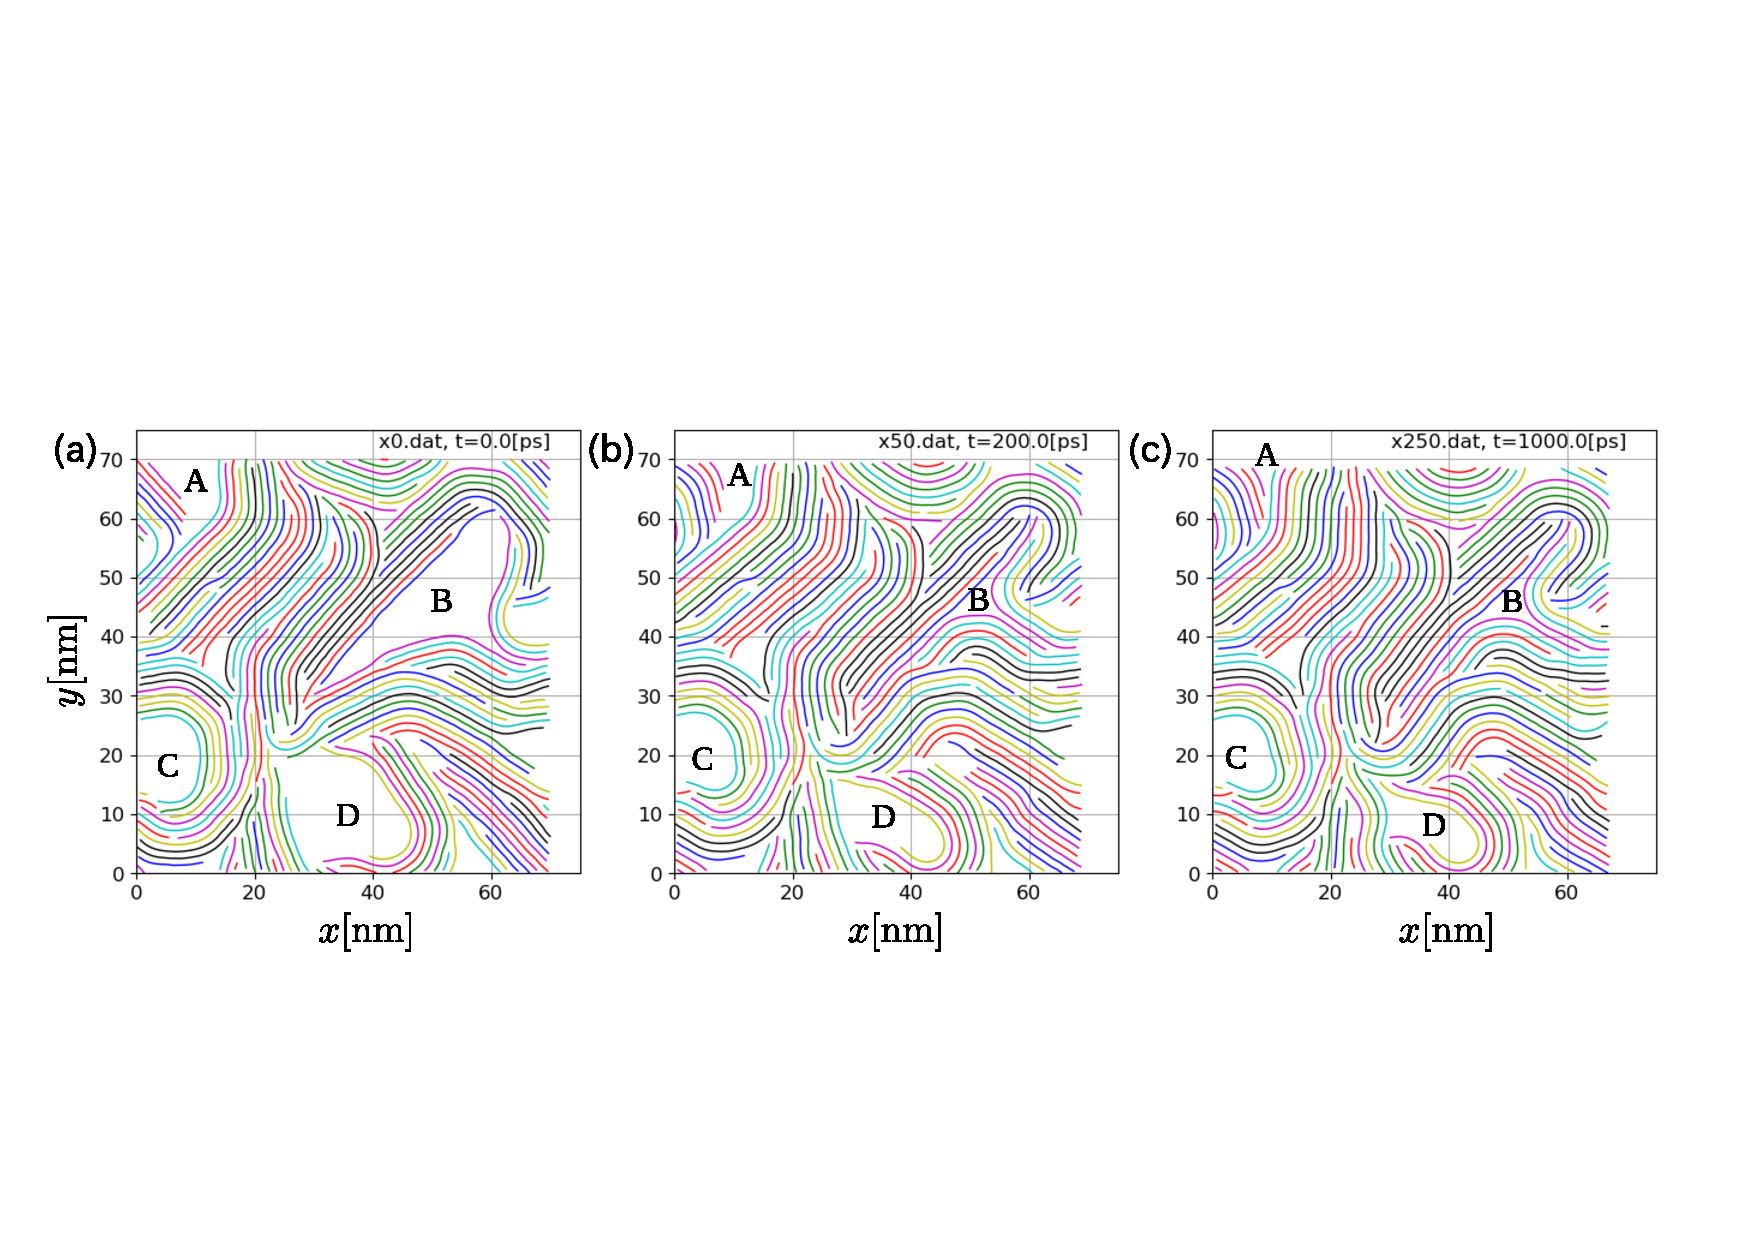
\includegraphics[width=1.0\linewidth]{Figs/fig3.pdf} 
	\end{center}
	\caption{
		相対湿度50$\%$での緩和にともなう粘土分子配置の変化.  
		(a)は初期状態,(b)緩和開始から200psの状態,(c)は1ns経過後の最終状態.
		A-Dのラベルは粘土層外の主要な空隙を示す.
	} 
	\label{fig:fig3}
\end{figure}
\subsection{相対湿度による組織構造の違い}
相対湿度50$\%$の場合に加えて,10,20,65,75および90$\%$で同様にして
緩和計算を行った結果を図\ref{fig:fi4}に示す.
相対湿度以外の計算条件は前項50$\%$の場合と同じである.\\
これらの結果のうち,相対湿度が最も低い(a)10$\%$のケースでは,
初期構造からあまり変化が見られず,層外間隙の形や大きさは
当初の状態と同程度のままになっている.これは,初期構造が
相対湿度が極めて低い場合に生じうるものであったことを意味する.
ただし,系全体の体積はやや収縮しており,若干の排水が起きている
ものと予想される.この次に低い湿度の(b)20$\%$では,全体の体積は
(a)と同程度の収縮となっているが,層外間隙は収縮が大きいものも
あり,相対湿度50$\%$によく似た分子配置となっている.
ただし(c)のケースよりも初期状態からの系全体の収縮量は
(b)の方が大きく,(b)から(c)の相対湿度範囲で排水から吸水が
進行し始めると解釈できる.これに対して(d)の65$\%$の場合,
全体としての体積変化はほぼ無視できる程度である一方,
粘土層間の距離は(c)の場合より大きく,明らかな吸水に
転じていることが分かる.この段階では粘土分子の巻き込み
で残留した層外空隙も,かなりの程度圧縮が進んでいる.
さらに相対湿度の高い(e)と(f)では,系全体としても膨張する
様子が見られ,このことは,層外間隙の体積収縮が(d)のケース
以上には進行していないことと呼応している.\\
%--------------------
\begin{figure}[h]
	\begin{center}
	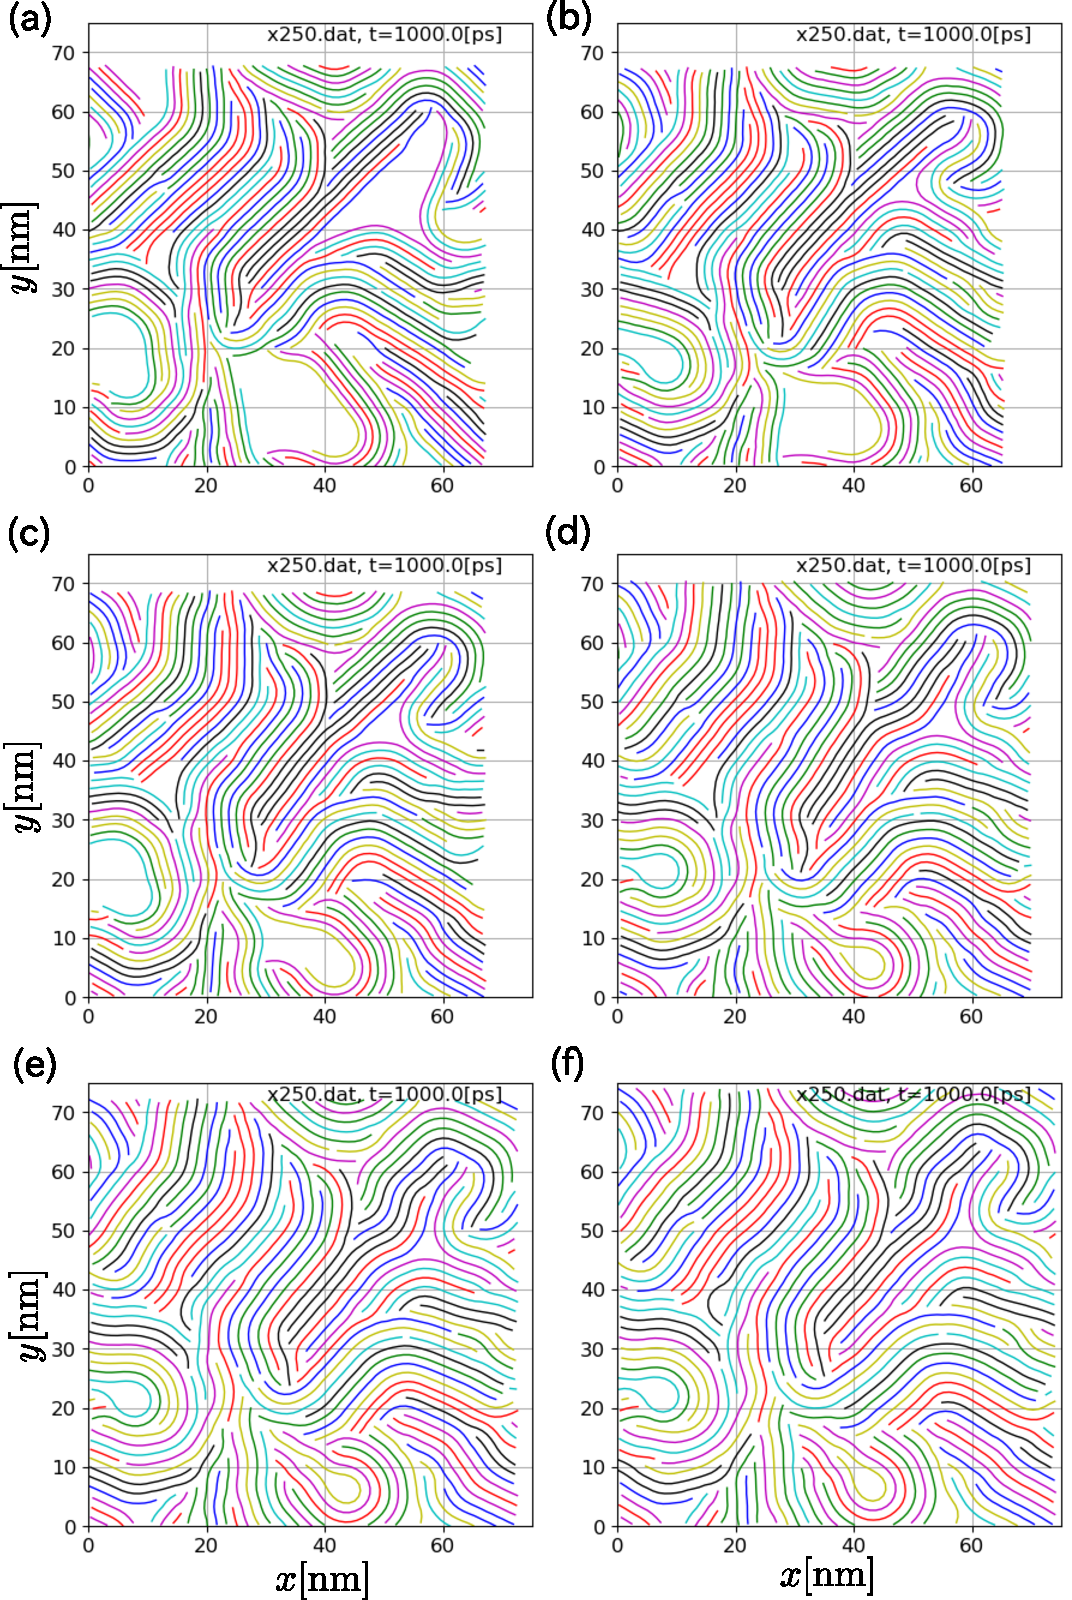
\includegraphics[width=0.8\linewidth]{Figs/fig4.pdf} 
	\end{center}
	\caption{
		6つの異なる相対湿度において得られた粘土含水系の組織構造.
		相対湿度は(a)から(f)の順に10,20,50,65,75および90$\%$. 
		相対湿度50$\%$の結果は,図\ref{fig:fig3}-(c)と同じものを再掲.
	} 
	\label{fig:fig4}
\end{figure}

相対湿度と膨潤状態の関係をより詳しく調べるために,層間距離の変化をみる.
図\ref{fig:fig5}はそのために,相対湿度毎に,層間距離の頻度分布を
示したもので,横軸は層間距離を縦軸は頻度を示している.
CG-MD法では,水分量を粒子間相互作用を規定するレナード-ジョーンズ
ポテンシャルの特性距離$\sigma$で表現している.$\sigma$は,概ね,
粘土分子が積層したときの層間距離となるため,$\sigma$を層間距離とみなし,
その頻度分布を描いたのが図\ref{fig:fig5}である.
横軸の範囲は,10から16$\AA$としており,図\ref{fig:fig1}-(a)からも明らかな
ように,液体の水に系が接触していない場合この範囲外の層間距離となることはない.
なお,無水状態である0膨潤では層間距離は約10$\AA$,1および2分子層膨潤ではそれぞれ
12.5と15.5$\AA$である。ただし,図\ref{fig:fig1}-(a)からも分かるように,
天然のモンモリロナイトでは離散的な膨潤状態とそれに対応す層間距離を
厳密に定義することは難しく,上に挙げた層間距離の値は代表値と考えることがより実情にあう.

図\ref{fig:fig5}からも,全体的な傾向としては相対湿度の増加にともない,
層間距離が大きくなることことは明らかである.
ただし,分布形状は相対湿度によって大きく異なり,
相対湿度が低い程分布幅が広い傾向があること,湿度によっては,2つあるいは
3つのピークを持つ分布となることが特徴として挙げられる.
また,一つ一つの分布に関して言えば以下のことが読み取れる.
相対湿度が最も低い(a)の結果は,他の場合よりも分布幅が明らかに広く,
層間距離は10$\sim$12$\AA$の間に分布し, 0層と1層膨潤の中間的な
状態となっている.この次に相対湿度の低い(b)の場合は,層間距離は
12$\AA$周辺に集中し,ほぼ1層膨潤状態に移行している.
図\ref{fig:fig1}-(a)を見ると,粉末X線回折試験では10$\sim$20$\%$の
相対湿度では0層膨潤となっているため,CG-MD計算の方が,
水分量が多い結果を与えている.これは,粘土分子の積層構造
に起因する差で,粉末状態よりも多くの水分を持つ方が,系全体の
自由エネルギーを下げ,構造を安定させるためと考えられる.
逆に言えば,指定された初期構造から0層膨潤状態に移行させるためには,
より大きなエネルギーを加えて計全体を強く圧縮するか,組織構造
を破壊する必要があることを示唆している.
これに対し,相対湿度50$\%$の結果(c)では,分布幅が狭く
層間距離がほぼ12.5$\AA$と決まる. これは粉末XRD試験の結果とも一致し,
系全体としても体積膨張を起こすことなく水分が取り込まれていることから,
無理のない状態,維持されやすい組織構造になっていると考えられる.
次に,(d)65$\%$と(e)75$\%$の結果を見ると,3つあるいは2つピークをもつ
多峰的な分布になっている.
粉末X線試験結果では,これらの湿度は1層から2膨潤への遷移領域にあたる.
13$\AA$と15.5$\AA$付近のピークは,これら2つの膨潤状態にそれぞれ対応
しており,Na型モンモリロナイトの膨潤挙動がよく現れている.
(d)では13$\AA$前後で2つの峰に分布が分かれている.
層間距離が大きい側の小ピークは既に2層へ移行が開始しているが、
十分な水分が行き渡らずに1層膨潤付近の層間距離にあるものと
考えられ,図\ref{fig:fig1}-(a)の膨潤曲線の折れ曲がりに対応している.
これよりもやや湿度の高い(e)のケースでは,1層から2層へ全て移行を
開始しており、その結果として13$\AA$以下のピークは完全に消失している.
最も高い湿度の(f)の場合は、2層膨潤への移行が終了し,
非常に鋭いピークを持つ分布が15.5$\AA$の位置に現れ,粉末X線回折試験
結果で観察される層間距離ともほとんど一致している.
なお,(d)に見られる第3の小ピークを伴う遷移挙動が実際の固体粘土で観察も
現れるのか,また組織構造との関連があるのかどうかは,固体粘土の組織構造を
理解する上で興味深い問題である。
以上に示した通り,今回のCG-MD計算に用いた水和エネルギーモデルでは,
Na型モンモリロナイトの離散的な膨潤挙動に見られる特徴を再現できること,
粉末X線回折試験では見られない組織構造に起因した挙動の双方が現れる
ことが分かる.
%--------------------
\begin{figure}[h]
	\begin{center}
	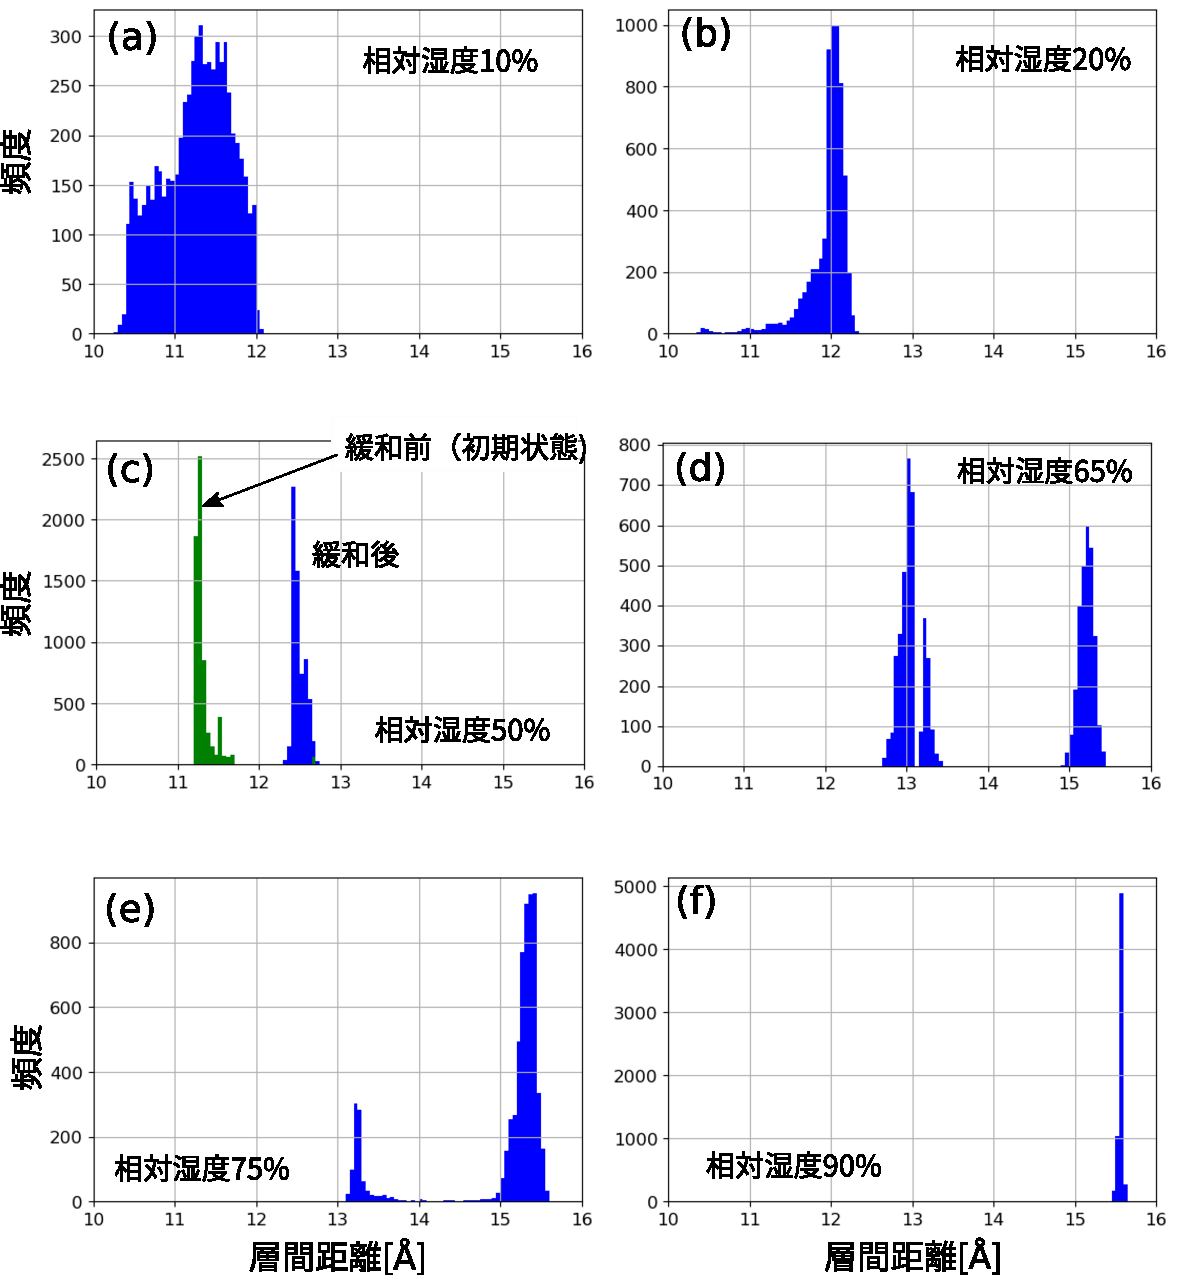
\includegraphics[width=1.0\linewidth]{Figs/fig5.pdf} 
	\end{center}
	\caption{
		6つの異なる相対湿度における,層間距離の頻度分布.
		相対湿度は(a)から(f)の順に10,20,50,65,75および90$\%$. 
	} 
	\label{fig:fig5}
\end{figure}
%--------------------
